\documentclass{article}\usepackage{graphicx, color}
%% maxwidth is the original width if it is less than linewidth
%% otherwise use linewidth (to make sure the graphics do not exceed the margin)
\makeatletter
\def\maxwidth{ %
  \ifdim\Gin@nat@width>\linewidth
    \linewidth
  \else
    \Gin@nat@width
  \fi
}
\makeatother

\definecolor{fgcolor}{rgb}{0.2, 0.2, 0.2}
\newcommand{\hlnumber}[1]{\textcolor[rgb]{0,0,0}{#1}}%
\newcommand{\hlfunctioncall}[1]{\textcolor[rgb]{0.501960784313725,0,0.329411764705882}{\textbf{#1}}}%
\newcommand{\hlstring}[1]{\textcolor[rgb]{0.6,0.6,1}{#1}}%
\newcommand{\hlkeyword}[1]{\textcolor[rgb]{0,0,0}{\textbf{#1}}}%
\newcommand{\hlargument}[1]{\textcolor[rgb]{0.690196078431373,0.250980392156863,0.0196078431372549}{#1}}%
\newcommand{\hlcomment}[1]{\textcolor[rgb]{0.180392156862745,0.6,0.341176470588235}{#1}}%
\newcommand{\hlroxygencomment}[1]{\textcolor[rgb]{0.43921568627451,0.47843137254902,0.701960784313725}{#1}}%
\newcommand{\hlformalargs}[1]{\textcolor[rgb]{0.690196078431373,0.250980392156863,0.0196078431372549}{#1}}%
\newcommand{\hleqformalargs}[1]{\textcolor[rgb]{0.690196078431373,0.250980392156863,0.0196078431372549}{#1}}%
\newcommand{\hlassignement}[1]{\textcolor[rgb]{0,0,0}{\textbf{#1}}}%
\newcommand{\hlpackage}[1]{\textcolor[rgb]{0.588235294117647,0.709803921568627,0.145098039215686}{#1}}%
\newcommand{\hlslot}[1]{\textit{#1}}%
\newcommand{\hlsymbol}[1]{\textcolor[rgb]{0,0,0}{#1}}%
\newcommand{\hlprompt}[1]{\textcolor[rgb]{0.2,0.2,0.2}{#1}}%

\usepackage{framed}
\makeatletter
\newenvironment{kframe}{%
 \def\at@end@of@kframe{}%
 \ifinner\ifhmode%
  \def\at@end@of@kframe{\end{minipage}}%
  \begin{minipage}{\columnwidth}%
 \fi\fi%
 \def\FrameCommand##1{\hskip\@totalleftmargin \hskip-\fboxsep
 \colorbox{shadecolor}{##1}\hskip-\fboxsep
     % There is no \\@totalrightmargin, so:
     \hskip-\linewidth \hskip-\@totalleftmargin \hskip\columnwidth}%
 \MakeFramed {\advance\hsize-\width
   \@totalleftmargin\z@ \linewidth\hsize
   \@setminipage}}%
 {\par\unskip\endMakeFramed%
 \at@end@of@kframe}
\makeatother

\definecolor{shadecolor}{rgb}{.97, .97, .97}
\definecolor{messagecolor}{rgb}{0, 0, 0}
\definecolor{warningcolor}{rgb}{1, 0, 1}
\definecolor{errorcolor}{rgb}{1, 0, 0}
\newenvironment{knitrout}{}{} % an empty environment to be redefined in TeX

\usepackage{alltt}
\usepackage{graphicx, color, amssymb, amsmath, bm, rotating, graphics,
epsfig, multicol, amsthm}
\usepackage{fullpage}
\usepackage[maxfloats=48]{morefloats} %for >18 figures
\usepackage{booktabs}
\usepackage{caption}
\usepackage[numbers]{natbib}
%Independent: use as X \ind Y | Z
\newcommand\ind{\protect\mathpalette{\protect\independenT}{\perp}}
\def\independenT#1#2{\mathrel{\rlap{$#1#2$}\mkern2mu{#1#2}}}
\newtheorem{alg}{Algorithm}
\newtheorem{theorem}{Theorem}
\IfFileExists{upquote.sty}{\usepackage{upquote}}{}
\begin{document}




\title{Ancillarity-Sufficiency or not; Interweaving to improve MCMC estimation of the local level DLM: Extended Abstract}
\author{{\bf Matthew Simpson}, Jarad Niemi and Vivekananda Roy}
\maketitle


MCMC estimation of the posterior density for dynamic linear models (DLMs) is often slow and computationally expensive. We explore the potential of the interweaving strategies of \cite{yu2011center} in order improve the speed of convergence to the stationary distribution in MCMC for DLMs, in particular the local level model. Let $\{y_t\}$ be a sequence of real valued random variables representing an observation for each period $t$, and let $\{\theta_t\}$ be another sequence of real valued random variables representing a latent state for each period.  The observations range from $t=1,...,T$ and the states range from $t=0,...,T$. We can write the model as
\begin{align*}
  y_t |\theta_{0:T}& \stackrel{ind}{\sim} N(\theta_t,V) \\
  \theta_t |\theta_{0:t-1}& \sim N(\theta_{t-1},W)
\end{align*}
for $t=1,2,...,T$ where $\theta_0\sim N(m_o,C_o)$. We refer to $v_t=y_t-\theta_t$ as the observation error and $w_t=\theta_t-\theta_{t-1}$ as the system disturbance. Here $(V,W)$ is the unknown parameter vector. A priori assume that $V$ and $W$ are independent with $V\sim IG(\alpha_V, \beta_V)$ and $W\sim IG(\alpha_W, \beta_W)$ where $\alpha_V$, $\beta_V$, $\alpha_W$, and $\beta_W$ are known hyperparameters.

The usual data augmentation (DA) algorithm for MCMC sampling from the posterior of the local level model, the state sampler, is a Gibbs sampler with two steps. First, draw $\theta_{0:T}$ from $p(\theta_{0:T}|V,W,y_{1:T})$ using the forward filtering backward sampling algorithm from \cite{fruhwirth1994data} and \cite{carter1994gibbs}. Second, draw $(V,W)$ from $p(V,W|\theta_{0:T}, y_{1:T})$ (from independent inverse gamma distributions). In some regions of the parameter space this algorithm runs into convergence and mixing problems. One tried and true method for dealing with this issue is reparameterization, in our case possibly of the augmented data vector. In the hierarchical models literature, for example, \cite{papaspiliopoulos2007general} describe the centered, noncentered and partially noncentered parameterizations. Some of these ideas are applied in the context of a particular DLM  --- a dynamic univariate regression with a stationary AR(1) regression coefficient --- in \cite{fruhwirth2004efficient}.

We introduce two more DA algorithms for MCMC sampling for the local level model: one based on the scaled disturbances, defined by $\gamma_0 = \theta_0$, and for $t=1,2,...,T$, $\gamma_t = (\theta_t - \theta_{t-1})/\sqrt{W}=w_t/\sqrt{W}$; and the other based on the scaled errors, defined by $\psi_0=\theta_0$, and for $t=1,2,...,T$, $\psi_t = (y_t - \theta_{t})/\sqrt{V}=v_t/\sqrt{V}$. The analogue of the scaled disturbances for a dynamic regression model are used in \cite{fruhwirth2004efficient}.

In addition we introduce several interweaving algorithms based on these DAs, applying the ideas of \cite{yu2011center}. A global interweaving strategy (GIS) inserts an additional step in the middle of the DA algorithm above to draw, e.g., $\gamma_{0:T}$ from $p(\gamma_{0:T}|\theta_{0:T},y_{1:T})$, then $(V,W)$ is drawn conditional on $\gamma_{0:T}$ instead of $\theta_{0:T}$. When $p(y_{1:T}|V,W,\theta_{0:T})$ is free of $(V,W)$, $\theta_{0:T}$ is called a sufficient augmentation (SA). When $p(\theta_{0:T}|V,W)$ is free of $(V,W)$, $\theta_{0:T}$ is called an ancillary augmentation (AA). Much of the promise of GIS comes from interweaving between a SA--AA pair. It turns out that $\gamma_{0:T}$ and $\psi_{0:T}$ are both AA's for $(V,W)$ but $\theta_{0:T}$ is not a SA nor an AA for $(V,W)$. We construct four GIS algorithms that interweave between any two or three of the three data augmentations discussed above. We also construct several algorithms using the component interweaving strategy (CIS). 

In order to test these algorithms, we simulated fake datasets over a grid in $V$--$W$ space and for $T=10$, $100$, and $1000$. Then we fit the local level model for each dataset using each sampler. We used the following priors: $\theta_0\sim N(0,10^7)$, $V\sim IG(5, 4V^*)$, and $W\sim IG(5, 4W^*)$,  independent where  $(V^*,W^*)$ are the true values of $V$ and $W$ used to simulate the time series. The chains were started at $(V^*,W^*)$.

Based on the simulations, the scaled disturbances and the scaled errors appear to make a great ``beauty and the beast'' pair for GIS --- they have good mixing for $(V,W)$ in opposite regions of the parameter space (see Figure \ref{plot}). This suggests they should combine well in an interweaving algorithm. The GIS algorithm based on the scaled disturbances and errors in fact has the best mixing properties: very good for both $V$ and $W$ when $W^*/V^*$ is far away from one, while when $T$ is large and $W^*/V^*$ is near one, mixing is poor for both $V$ and $W$. Figure \ref{plot} illustrates the improvement in mixing by using the GIS sampler instead of either of the two underlying DA algorithms and the improvement over the state sampler. In addition, we find that the GIS algorithms seem to have identical mixing to their corresponding alternating algorithms and to the CIS algorithms, where another sort of correspondence holds. GIS is cheaper than both computationally, so it has the advantage.

These results are not ideal in that the algorithm which seems to work best, the disturbance-error GIS algorithm, still has poor mixing for large $T$ when $W^*/V^*$ isn't too far from one, i.e. the most commonly encountered region of the parameter space. It is an improvement, however, and the results point to generalizations for more complicated DLMs. 





\begin{knitrout}
\definecolor{shadecolor}{rgb}{0.969, 0.969, 0.969}\color{fgcolor}\begin{figure}[!ht]


{\centering 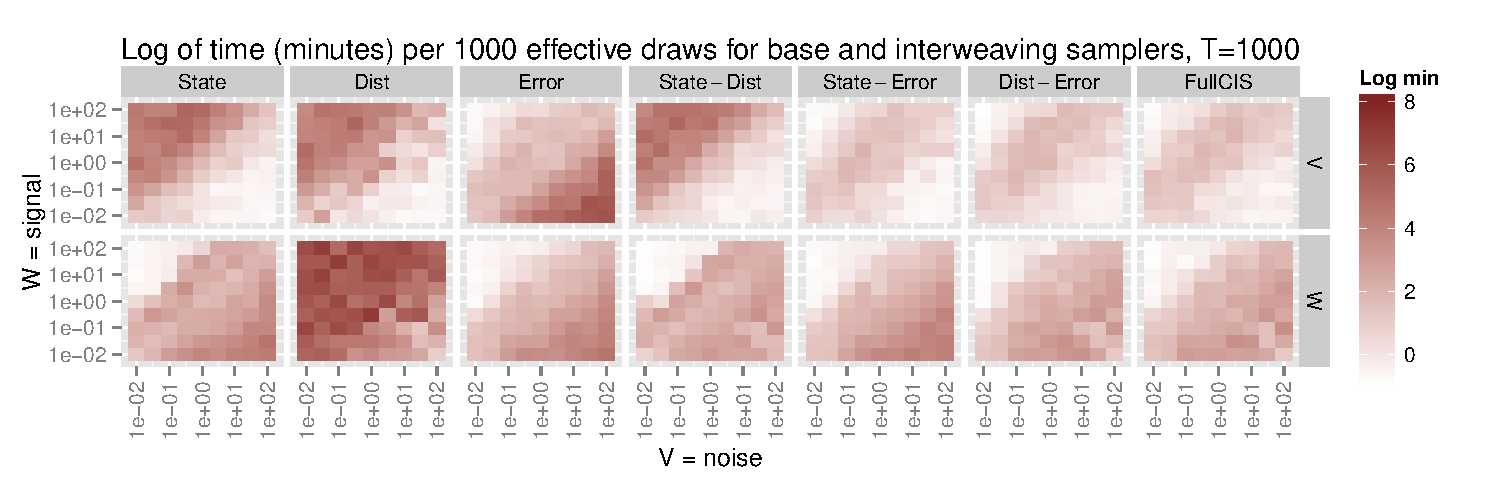
\includegraphics[width=.75\textwidth]{figure/plot} 

}

\caption[\footnotesize Effective sample size as a proportion of the actual sample size for $V$ and $W$ in each posterior sampler for $T=100$ in the state, scaled disturbance and scaled error samplers and for all three GIS samplers based on any two of these]{\footnotesize Effective sample size as a proportion of the actual sample size for $V$ and $W$ in each posterior sampler for $T=100$ in the state, scaled disturbance and scaled error samplers and for all three GIS samplers based on any two of these. Horizontal and vertical axes indicate the true values of $V$ and $W$ respectively for the simulated data. Note that the signal-to-noise ratio is constant moving up any diagonal. In the upper left the signal is high, in the lower right the noise is high. Also note that for plotting purposes, effective sample proportions larger than one were rounded down to one.\label{plot}}
\end{figure}


\end{knitrout}


\bibliographystyle{plainnat}
\bibliography{../mcmcex}
\end{document}
